% Kompiuterijos katedros šablonas
% Template of Department of Computer Science II
% Versija 1.0 2015 m. kovas [ March, 2015]

\documentclass[a4paper,12pt,fleqn]{article}
\usepackage[unicode,colorlinks=false]{hyperref}


\usepackage[utf8x]{inputenc}
%

\usepackage[L7x]{fontenc}
\usepackage{times}
\usepackage{ucs}
\usepackage{tabto}

 %package to switch the languageja
\usepackage{etoolbox}

  %set up of the page margins
\usepackage[top=2cm, bottom=2cm, left=3cm, right=1.5cm]{geometry}

 %1.1 line spacing
\linespread{1.1}


  %page numbering at the right side
\usepackage{fancyhdr}
\pagestyle{fancyplain}
\fancyhf{}
\renewcommand{\headrulewidth}{0pt} 
\fancyhfoffset[RO]{0cm}

  %to number at the bottom (exchange lines to number at the top)
\rfoot{\thepage}
  %\rhead{\thepage} %

% \usepackage[usenames,dvipsnames]{pstricks}
\urlstyle{same}
\hypersetup{
%  citecolor=Blue,
%  linkcolor=Blue,
%  urlcolor=Blue
pdfborder={0 0 0 }
}

 %for includegraphics
\usepackage{graphicx}



\usepackage[toc,page]{appendix}


\usepackage{caption}

 %for source codes
\usepackage{listings}
\lstset{commentstyle=\color{red},xleftmargin=10pt, framexleftmargin=6pt, numbersep=1mm, frame=single, numbers=left,numberstyle=\footnotesize,extendedchars=\true, inputencoding=utf8x,basicstyle=\footnotesize,extendedchars=true,
 keywordstyle=\color{black}\bfseries, breaklines=true, breakautoindent=true,framesep=8pt,linewidth=0.95\textwidth
}

 %for algorithms
\usepackage{algorithm}
\usepackage{algorithmic}
 %instead of the above two packages we can use algorithms2e
 %\usepackage[boxed,linesnumbered,vlined,slide]{algorithm2e}

 %special symbols
\usepackage{amsfonts}
\usepackage{amssymb}
\usepackage{amsmath}

 %for theorem like environments
\usepackage{amsthm}

 \usepackage{datetime}
 \renewcommand{\dateseparator}{--}


% SI system units
\usepackage{siunitx}
\sisetup{detect-all}
% Problem with fonts \SI{x.xx}{\micro\metre}, solved with updmap-sys --enable Map=utm.map
\renewcommand{\sfdefault}{uhv}
\renewcommand{\rmdefault}{utm}
\renewcommand{\ttdefault}{ucr}

% List management (itemize, etc.)
\usepackage{enumitem}

\newcommand*{\urlw}[1]{\href{#1}%
            {\nolinkurl{#1}}}

\numberwithin{equation}{section}

\usepackage{tabu}
% \documentclass{article}
\usepackage[utf8]{inputenc}
\newcolumntype{P}[1]{>{\RaggedRight\arraybackslash}p{#1}}
\newcommand{\tabitem}{\textbullet~~}
\newtoggle{inLithuanian}
 %If the report is in Lithuanian, it is set to true; otherwise, change to false
\settoggle{inLithuanian}{true}
\newtheorem{exmp}{Example}[subsection]
\usepackage{tabularx}
\usepackage{listings}
\usepackage{tabu}
\usepackage{hyperref}
%create file preface.tex for the preface text
%if preface is needed set to true
\newtoggle{needPreface}
\settoggle{needPreface}{false}

\newtoggle{signaturesOnTitlePage}
\settoggle{signaturesOnTitlePage}{true}

\theoremstyle{definition}
\newtheorem{definition}{\keyWordDefinition}
\newtheorem{example}{\keyWordExample}
\def\QED{\unskip\nobreak\hfill\kern5pt$\Box$}

\iftoggle{inLithuanian}{
%\usepackage[L7x]{fontenc}
\usepackage[english,lithuanian]{babel}
\usepackage{tabu}
\newcommand{\todayiso}{\the\year \dateseparator \twodigit\month \dateseparator \twodigit\day}



\renewcommand{\today}{\number\year\space m. \space \ifcase\month\or
  sausio\or vasario\or kovo\or balandžio\or gegužės\or birželio\or
  liepos\or rugpjūčio\or rugsėjo\or spalio\or lapkričio\or
  gruodžio\fi
  \space\number\day\space d.}


 \usepackage{tocloft}
 \renewcommand\cftsecaftersnum{.} 
 \renewcommand\cftsubsecaftersnum{.} 
 \renewcommand\cftsubsubsecaftersnum{.}

 \usepackage{VUMIFKK}

 \DeclareCaptionLabelFormat{captionlt}{#2 #1}
   %smth is not fine with algorithms 
 \DeclareCaptionLabelFormat{captionltalg}{#2 #1 algoritmas}

 \usepackage{indentfirst}
 \renewcommand{\appendixtocname}{Priedai}
 \renewcommand{\appendixpagename}{Priedai}
 \renewcommand{\contentsname}{Turinys} 

 \renewcommand{\lstlistingname}{išeities kodas}
 \renewcommand{\figurename}{pav}
 \renewcommand{\tablename}{lentelė}


 \captionsetup*[lstlisting]{   
 labelsep=period,labelformat=captionlt
 }
 \captionsetup*[figure]{   
% labelsep=period,
 labelsep=space, %babel redefines pav to pav.
 labelformat=captionlt
 }
 \captionsetup*[table]{   
  labelsep=period,
  labelformat=captionlt
 }
 \renewcommand{\algorithmicrequire}{\textbf{Įvestis:}}
 \renewcommand{\algorithmicensure}{\textbf{Išvestis:}}

 \captionsetup*[algorithm]{   
 labelsep=period,labelformat=captionltalg
 }

\renewcommand{\thmhead}[3]{#2 #1#3}

}
{
%\usepackage[OT1,T1]{fontenc}
%\usepackage[L7x]{fontenc}



\usepackage[english]{babel}
\newcommand{\todayiso}{\twodigit\month \dateseparator \twodigit\day \dateseparator \the\year}
 \captionsetup*[algorithm]{   
 labelsep=period
 }
\captionsetup*[lstlisting]{   
 labelsep=period
 }
 \captionsetup*[figure]{   
 labelsep=period
 }
 \captionsetup*[table]{   
 labelsep=period
 }


}

%some kywords
 \def\keywordAbstract{\iftoggle{inLithuanian}{Santrauka}{Abstract}}
 \def\keywordAbstractOther{\iftoggle{inLithuanian}{Summary}{Santrauka}}
 \def\keyWordIntroduction{\iftoggle{inLithuanian}{Įvadas}{Introduction}}
 \def\keyWordConclusions{\iftoggle{inLithuanian}{Išvados ir rekomendacijos}{Conclusions and Recommendations}}

 \def\keyWordPreface{\iftoggle{inLithuanian}{Pratarmė}{Preface}}
 \def\keyWordAppendice{\iftoggle{inLithuanian}{Priedas}{Appendix}}
 \def\keyWordSignature{\iftoggle{inLithuanian}{parašas}{signature}}
 \def\keyWordDefinition{\iftoggle{inLithuanian}{apibrėžimas}{Definition}}
 \def\keyWordExample{\iftoggle{inLithuanian}{pavyzdys}{Example}}

\newcommand{\bothabstracts}[3]{
\setcounter{secnumdepth}{0}
\newpage
\hspace{2cm}
{\centering{\section{\keywordAbstract}}}

#1
\newpage
\hspace{2cm}
{\centering \section{\keywordAbstractOther}}

\begin{center}{\textbf{#2} }\end{center}

 #3
\setcounter{secnumdepth}{3}
}

 %non-numbered sections: #1 param: for labeling sec:#1, #2 -section title
\newcommand{\sectionWithoutNumber}[2]{\newpage
%\hspace{2cm}
\section*{#1}
\label{sec:#2}
\addcontentsline{toc}{section}{\nameref{sec:#2}}%{#3}
 }



\newcommand{\referenceSources}[1]{
\newpage
\cleardoublepage
\phantomsection
\iftoggle{inLithuanian}{
 \renewcommand{\refname}{Literatūros šaltiniai}

 \addcontentsline{toc}{section}{Literatūros šaltiniai}
 \markboth{\refname}{Literatūros šaltiniai}
 }
{

\addcontentsline{toc}{section}{References}
\markboth{References}{References}
}

\bibliographystyle{plain}
\bibliography{#1}
}



 \newcommand\authorsignature[1]{
\begin{flushright}
 \begin{minipage}[b]{0.45\textwidth}
  \centering
  \rule{\textwidth}{0.5pt}\\
   #1
  \end{minipage}
\end{flushright}
 }




 \newcommand\authorsignatures[5]{%
   \vspace{1cm}
   \authorsignature{#1}
   \ifstrequal{#2}{}{}{\vspace{0.3cm}
     \authorsignature{#2}
     \ifstrequal{#3}{}{}{\vspace{0.3cm}
      \authorsignature{#3}
      \ifstrequal{#4}{}{}{\vspace{0.3cm}
        \authorsignature{#4}
        \ifstrequal{#5}{}{}{\vspace{0.3cm}
         \authorsignature{#5}       
        }
      }
    }
} 
}

\newcommand{\authortitle}{
\iftoggle{signaturesOnTitlePage}{
\tiny{\keyWordSignature}
}{}
}

\newcommand{\depttitlepage}[8]
{
\thispagestyle{empty}
\begin{center}


\includegraphics[width=2cm]{jb_VU_zenklas}

%\vspace{-1cm}

\iftoggle{inLithuanian}
{ 
  VILNIAUS UNIVERSITETAS\\
  MATEMATIKOS IR INFORMATIKOS FAKULTETAS\\
  INFORMATIKOS INSTITUTAS\\
  KOMPIUTERINIO IR DUOMENŲ MODELIAVIMO KATEDRA
}
{
  VILNIUS UNIVERSITY \\
  FACULTY OF MATHEMATICS AND INFORMATICS \\
  INSTITUTE OF COMPUTER SCIENCE\\
  DEPARTMENT OF COMPUTATIONAL AND DATA MODELING
}

\vspace{5cm}

#1\\
\vspace{0.5cm}
\textbf{\Large #2}
\end{center}

\vspace{5cm}


\hspace{0.5\textwidth}
\begin{minipage}{0.4\textwidth}
 \begin{flushleft} 
\iftoggle{inLithuanian}
{
 \ifstrequal{#3}{}{}{Atliko:\\[5pt]}
}
{
\ifstrequal{#3}{}{}{Done by:\\[5pt]}
}

%\noindent
\begin{tabular}{@{}lr}%\setlength\tabcolsep{0pt}
\ifstrequal{#3}{}{}{#3&\hspace{2cm}\authortitle\\[5pt]}
\ifstrequal{#4}{}{}{#4&\authortitle\\[5pt]}
\ifstrequal{#5}{}{}{#5&\authortitle\\[5pt]}
\ifstrequal{#6}{}{}{#6&\authortitle\\[5pt]}
\ifstrequal{#7}{}{}{#7&\authortitle\\}
\end{tabular}

\end{flushleft}

\end{minipage}

\vspace{0.5cm}
\hspace{0.5\textwidth}
\begin{minipage}{0.4\textwidth}
 \begin{flushleft} 

\ifstrequal{#8}{}{}
{

\iftoggle{inLithuanian}
{
Vadovas:
}
{
Supervisor:
}

#8

}

\end{flushleft}

\end{minipage}


\vfill

\begin{center}
Vilnius\\
\the\year
\end{center}

\iftoggle{needPreface}{
 \sectionWithoutNumber{\keyWordPreface}{preface}
Pratarmės (Preface) informacija


\iftoggle{inLithuanian}
{
\vspace{\baselineskip}\hfill
\today
}
{
 \vspace{\baselineskip}\hfill \today
}

 \vspace{5cm}

\iftoggle{signaturesOnTitlePage}{}
{
\authorsignatures{#3}{#4}{#5}{#6}{#7}
}
}{}
\newpage
}


\usepackage{listings}
\usepackage{color}

\definecolor{dkgreen}{rgb}{0,0.6,0}
\definecolor{gray}{rgb}{0.5,0.5,0.5}
\definecolor{mauve}{rgb}{0.58,0,0.82}

\lstset{frame=tb,
  language=Java,
  aboveskip=1mm,
  belowskip=1mm,
  showstringspaces=false,
  columns=flexible,
  basicstyle={\small\ttfamily},
  numbers=none,
  numberstyle=\tiny\color{gray},
  keywordstyle=\color{blue},
  commentstyle=\color{dkgreen},
  stringstyle=\color{mauve},
  breaklines=true,
  breakatwhitespace=true,
  tabsize=3
}

\begin{document}
 % #1 -report type, #2 - title, #3-7 students, #8 - supervisor
 \depttitlepage{Kursinis darbas}{Automatinio testavimo metodologijų tyrimas}{Adomas Bazinys} 
 {}{}{}{}% students 2-5
 {Dr. Joana Katina}

\tableofcontents

 %both abstracts
\bothabstracts{Per pastaruosius 30 metų programinės įrangos pramonė padarė didelę pažangą ir pakeitė daugelio žmonių gyvenimą. Šiais laikais skambinant, užvedant automobilį, įjungiant elektrinę viryklę, atsiskaitant debeto kortele, daugelis net nenumanome, kad tokių procesų metu vykdome tam tikrą programinės įrangos kodą. Paprastai programinė įranga susiduria su dvejais iššūkiais: kuo mažesnės programavimo darbų išlaidos ir produkto kokybės užtikrinimas. Kokybiška programinė įranga gali būti apibūdinama kaip naudinga, patikima ir saugi programinė įranga. Programinės įrangos kokybė turi įtakos pasaulio ekonomikai, nacionaliniam saugumui, sveikatos priežiūrai, todėl programinės įrangos kokybė yra didžiulė atsakomybė. Šis darbas yra orientuotas į internetinių aplikacijų kokybę bei turi tikslą atsakyti į klausimą, kaip automatinis testavimas gali prisidėti prie internetinių aplikacijų kokybės.}%tex-file of abstract in original language
{Automated Testing Frameworks Reliability Impact on Web Application Development Life Cycle} %if work is in LT this title should be in English
{Over the last 30 years, the software industry has made great progress and has changed the lives of many people. Nowadays, when calling a phone, starting a car, switching on an electric stove, making a debit card payment we do not even think that during such a processes we run a certain program code. Typically, software has to overcome two challenges: reduce the cost of development as possible and ensure the high quality. High quality software can be described as usable, dependable, and safe software. Software quality affects the global economy, national security, health, safety, so software quality is a huge responsibility. This work is focused on the quality of web applications and will try to answer the question of how automated testing can contribute to software quality.}%tex-file of abstract in other language


%keywords and notations if needed
\sectionWithoutNumber{Trumpinių sąrašas}{keywords}{\begin{flushleft}
\textbf{ODBC} - Open Database Connectivity.
\newline
\newline
\textbf{CSV} - Comma Separated Values.
\newline
\newline
\textbf{SQL} - Structured Query Language.
\newline
\newline
\textbf{SUT} - System Under Test.
\end{flushleft}}


 %Introduction section: label is sec:intro
\sectionWithoutNumber{\keyWordIntroduction}{intro}
Didėjant WEB aplikacijos apimčiai ir naudotojų kiekiui, tampa vis sunkiau užtikrinti sistemos kokybę rankiniu būdu ir nepriekaištingas kokybės užtikrinimo procesas tampa neatskiriama aplikacijos vystymo dalimi. Tokiu atveju rankinis testavimas atsiranda poreikis naudoti automatinį testavimą.

Atliekant kodo pertvarkymą (\textbf{angl.} refactoring) arba naujų funkcijų įgyveninimą dažnai klaidos aptinkamos jau egzistuojančiuose kodo vienetuose. Tai gali padaryti didžiulę įtaką būsimo produkto kokybei, todėl testavimas turi būti pradedamas jau ankstyvoje programinės įrangos vystymosi ciklo stadijoje. Automatinis testavimas yra efektyvus būdas patikrinti aplikacijos kokybę prieš išleidžiant ją į produkciją.

Šio darbo tikslas yra išsiaiškinti ir pagrįsti kodėl ir kuris automatinio testavimo tipas yra efektyviausias, patikimiausias, bei turintis aukščiausią pakartotinio panaudojimo (\textbf{angl.} reusability) lygį. Bus rašomi testai, naudojant ir išbandant kiekvieną egzistuojantį automatinio testavimo tipą ir samprotaujama, kuris iš jų labiausiai atitinka paminėtus kriterijus. Pavyzdžiam bus naudojama JAVA programavimo kalba ir Selenium bei Cucumber testavimo karkasai.

\newpage
\section{Įvadas į testavimą}
Daugelis programuotojų tikriausiai sutiktų, kad defektai aplikacijoje dažnai atsiranda ne tik ją kuriant, bet ir išleidus ją į produkciją. Tikimybę sumažinti defektų skaičių padeda automatinis testavimas ~\cite{huizinga2007automated}.

Automatinis aplikacijų testavimas paprastai yra atliekamas rašant ir vykdant tam tikrus kodo vienetus, vadinamus testais. Kiekvienas testas naudoja jau egzistuojančią funkciją, kurią norima ištestuoti. Pagrindinis šio testavimo tikslas yra užtikrinti, kad gaunamas rezultatas yra toks, kokio tikimasi.

Kai kurios programavimo kalbos testavimui turi tam tikrus \textbf{assert} metodus, kurie tikrina, ar sąlyga yra teisinga - kitu atveju grąžina pranešimą apie įvykusią klaidą. Tačiau vien to testavimui neužtenka. Pavyzdžiui, mes norime paleisti tam tikrą kodo dalį prieš vykdant kiekvieną testą, taip pat, kad būtų grąžinamas tikslus pranešimas apie tai, kur yra klaida ir kodėl ji įvyko. Tai yra priežastys, kodėl testavime yra reikalingas testavimo karkasas (\textbf{liet.} testing framework) ~\cite{inproceedings}.

\subsection{Defekto apibrėžimas}
Svarbu suprasti, kad ne kiekviena problema aplikacijoje yra defektas. Defektas yra problema, kuri apriboja aplikacijos funkcionalumą arba neatitinka kliento reikalavimų. Jei aplikacija veikia tinkamai ir atitinka kliento poreikius, galima teigti, kad ji neturi defektų ~\cite{article}.

\subsection{Rankinis testavimas}
Rankinis testavimas yra primytiviausias testavimo būdas, kai testuotojas testavimo scenarijus vykdo rankiniu būdu - nenaudodamas jokių testų automatizacijai skirtų įrankių. Rankinio testavimo specialistas paprastai atlieka galutinio vartotojo vaidmenį, siekiant įsitikinti, ar visos tinklalapio funkcijos veikia taip, kaip tikimasi. Rankinis testuotojas dažnai vadovaujasi testavimo planu, į kurį yra įtraukti svarbiausi testavimo scenarijai ~\cite{itkonen2007defect}.

\subsubsection{Privalumai}
\begin{itemize}
    \item Nereikia programavimo kalbos žinių.
    \item Puikiai tinkamas būdas testuoti nedidelės apimties aplikacijas.
\end{itemize}

\subsubsection{Trūkumai}
\begin{itemize}
    \item Neefektyvu, reikalauja daug laiko.
    \item Sunkiai vykdomas regresinis testavimas.
    \item Neįmanoma pratestuoti aplikacijos greitaveikos (\textbf{angl.} performance).
\end{itemize}

\subsection{Automatinis testavimas}
Automatinis testavimas yra testavimo būdas, kai yra rašomi testavimo skriptai, naudojantis kokia nors programavimo kalba ar įrankiu, atliekantys tam tikrus paspaudimus grafinėje sąsajoje ir fiksuojantys testų rezultatus.

\subsubsection{Privalumai}
\begin{itemize}
    \item Lengva atlikti regresinį testavimą.
    \item Patogus, automatiškai atliekamas rezultatų apibendrinimas.
    \item Parašius testavimo skriptą, testavimo procesas tampa daug efektyvesnis.
\end{itemize}

\subsubsection{Trūkumai}
\begin{itemize}
    \item Būtinos bent vienos programavimo kalbos žinios.
\end{itemize}

\section{WEB aplikacijos plėtojimo ciklas}
Kuriant WEB aplikaciją, būtina remtis ir sekti tam tikrą vystymo metodologiją, norint užtikrinti nuoseklumą ir užbaigtumą. WEB aplikacijos vystymosi ciklas susideda iš kelių fazių ~\cite{french1970web}:

\begin{enumerate}
    \item Planavimas.
    \item Analizė.
    \item Plėtojimas.
    \item Testavimas.
    \item Paleidimas ir palaikymas.
\end{enumerate}

% https://www.academia.edu/37441077/Overview_of_Web_Development_Life_cycle_in_Software_Engineering
\subsection{Planavimas}
Pati pirmoji WEB aplikacijos plėtojimo ciklo fazė yra planavimas. Jei planavimo fazė yra praleidžiama arba į ją žiūrima atmestinai, tada visos sekančios fazės užtikrintai bus taip pat nenusisekusios, o tai reikštų projekto žlugimą ~\cite{french1970web}. Į planavimą įeina:

\begin{itemize}
    \item Apsisprendimas, kokias technologijas naudoti.
    \item Projekto tikslo apibrėžimas.
    \item Tikslinės grupės apibrėžimas.
    \item Nustatymas, kokį turinį aplikacija talpins.
\end{itemize}

\subsection{Analizė}
Tai yra fazė, kuomet analitikas renka informaciją apie reikalvimus, sistemingai juos analizuoja ir aprašo aplikacijos funkcionalumą pagal surinktą informaciją. Taip pat šioje stadijoje yra renkama informacija apie kliento lūkesčius greitaveikai (\textbf{angl.} performance), serverio atsako laikui (\textbf{angl.} response time) ir panašiai ~\cite{french1970web}.

\subsection{Plėtojimas}
Šioje fazėje yra sukuriama pati WEB aplikacija. Programuotojai ir dizaineriai paverčia ankstensėse fazėse sukurtą sistemos modelį į pilnai funkcionuojančią aplikaciją ~\cite{french1970web}.

\subsection{Testavimas}
Testavimas yra pati svarbiausia WEB aplikacijos vystymo ciklo dalis. Šioje fazėje lyginame, ar esamas funkcionalumas yra toks pats kaip ir funkcionalumas, kurio yra tikimasi. Jei skirtumo tarp šių funkcionalumų nėra, galime laikyti, kad sukurtas produktas yra kokybiškas ir atitinkantis kliento reikalavimus ~\cite{french1970web}. Į šią fazę taip pat įeina tokie patikrinimai kaip:

\begin{itemize}
    \item Nuorodų WEB aplikacijoje veikimas.
    \item Serverio atsako laikas. 
    \item WEB aplikacijos veikimas skirtingose naršyklėse.
    \item Žmogaus Kompiuterio sąveika.
    \item Validacijos.
    \item WEB aplikacijos paleidimas įvairiuose įrenginiuose: telefonai, planšetės ir t.t.
\end{itemize}

\subsection{Paleidimas ir palaikymas}
Į šią fazę įeina WEB aplikacijos, duomenų bazių valdymo sistemos paleidimas į produkciją, kad produktu galėtų naudotis tikslinis vartotojas ~\cite{french1970web}. Šioje fazėje atliekamos tokios užduotys, kaip:

\begin{itemize}
    \item Paleidimas į produkciją.
    \item Turinio atnaujinimas.
    \item Sistemos stebėsena.
    \item Informacijos apie lankytojus registravimas (\textbf{angl.} logging).
\end{itemize}

% https://www.softwaretestingmaterial.com/types-test-automation-frameworks/
\section{Automatinio testavimo karkasų tipai}
Automatinio testavimo karkasas yra rinkinys įrankių ir taisyklių, skirtų testavimo scenarijų kūrimui. Tai yra automatizuoto testavimo dalis, kuri padeda testuotojams efektyviau naudoti išteklius ir palengvina jų darbą.

\subsection{„Linear Scripting“ testavimas}
Ši testavimo metodika dar kitaip vadinamas "Įrašyk ir Atkurk" (\textbf{angl.} "Record and Playback") karkasu. Ji naudojamas testuoti nedidelės apimties WEB aplikacijoms. Naudojant šį testavimo būdą yra galimybė sugeneruoti testavimo skriptą neskiriant tam daug laiko, tačiau tai turi labai didelių trūkumų kaip pakartotinio panaudojamumo (\textbf{angl.} reusability) trūkumas, į testavimo skriptą įkoduotos reikšmės, kas neleidžia vykdyti scenarijaus naudojant kitus duomenis ar jų rinkinius. Šiam testavimo būdui praktiškai nereikalingos jokios programavimo žinios, norint testuoti šiuo būdu tereikia savo kompiuterio naršyklėje susinstaliuoti papildinius, tokius kaip Selenium ID, Katalon Recorder arba Robot Framework ir įrašinėti tam tikras veiksmų sekas galutiniame rezultate sugeneruojant testavimo scenarijaus skriptą norima kalba ~\cite{meszaros2003agile}.

\subsection{Ištrauka iš sugeneruoto "Record and Playback" skripto}
\begin{lstlisting}[caption={"Record and Playback" tipo testas.}]
click on linkText=Register OK
click on id=gender-male OK
click on id=FirstName OK
type on id=FirstName with value Tomas OK
click on id=LastName OK
type on id=LastName with value Tomaitis OK
click on name=DateOfBirthDay OK
select on name=DateOfBirthDay with value label=9 OK
click on name=DateOfBirthDay OK
click on name=DateOfBirthMonth OK
select on name=DateOfBirthMonth with value label=March OK
click on name=DateOfBirthMonth OK
click on css=.fieldset:nth-child(1) > .form-fields OK
click on name=DateOfBirthYear OK
select on name=DateOfBirthYear with value label=1997 OK
click on name=DateOfBirthYear OK
click on id=Email OK
type on id=Email with value adomas.adomaitis@gmail.com OK
click on id=Company OK
type on id=Company with value Company OK
click on css=.fieldset:nth-child(4) > .form-fields OK
click on id=Password OK
type on id=Password with value password OK
click on id=ConfirmPassword OK
type on id=ConfirmPassword with value password OK
click on css=.page-body > form OK
click on id=register-button OK
\end{lstlisting}
Šį Selenium IDE sugeneruotą skriptą konvertuoti į JAVA programavimo kalbą ir sėkmingai pasileisti.

\subsection{„Modularity Driven“ testavimas}
Daugelyje WEB aplikacijų egzistuoja funkcijos, kurios yra dažnai kartojamos ir priklausomos nuo kitų funkcijos. Ši testavimo metodika yra paremtas modulinėmis klasėmis, kuriose saugomi tam tikros funkcijos iškvietimo metodai. Tam, kad kiekvieną kartą neapsirašinėti kažkokios WEB puslapio funkcijos iškvietimo, modulinėje klasėje yra naudinga apsirašyti metodą ir esant poreikiui jį išsikviesti. Tai vadinama moduliškumu (\textbf{angl.} modularity). Norint atlikti pakeitimą tam tikros funkcijos iškvietime, užtenkta tik pakeisti metodą, iškviečiantį WEB puslapio funkciją. Metodas gali būti iškviečiamas keliose vietose, todėl šio testavimo tipo nauda ta, kad nereikia keisti to pačio kodo keliose vietose. Tai sumažina kodo duplikaciją ir palaiko "švarią" testinio kodo struktūrą ~\cite{kelly2003choosing}.

\newpage
\subsubsection{Modelinės klasės pavyzdys}
\begin{lstlisting}[caption={Testavimo naudojant modulius pavyzdys - modelinė klasė.}]
    public class PriceFilterModule {
    ...
    @FindBy(linkText = "Padangos")
    private WebElement tiresCat;

    @FindBy(linkText = "Vasarinės padangos")
    private WebElement summerTiresCat;

    public void chooseTiresCategory() {
        tiresCat.click();
    }

    public void chooseSummerTiresCategory() {
        summerTiresCat.click();
    }

    public boolean doesItemsCorrespondToPriceRange() throws IOException {
        for (int i = 0; i < fetchItemsPrices().size(); i++) {
            Double checkingValue = fetchItemsPrices().get(i);
            if (!(FilteringConstants.MIN_PRICE < checkingValue && checkingValue < FilteringConstants.MAX_PRICE)) {
                return false;
            }
        }
        return true;
    }
    ...
    }
\end{lstlisting}

Šis metodas tiesioginės įtakos produkto kokybei nedaro, tačiau turi įtakos teisingai ir "švariai" testavimo scenarijų kodo struktūrai. Ji daro įtaką atliekamų testų kokybei, kurie parodydami teigiamą rezultatą suklaidina testuotoją ir produktas prieš išleidžiamas į produkciją nėra kokybiškai ištestuojamas.

\newpage
\subsubsection{Testinės klasės pavyzdys}
\begin{lstlisting}[caption={Testinė klasė, kviečianti modulines klases.}]
public class PriceFilterModuleTest extends BaseTest {

    private HomePageModule homePageModule;
    private PriceFilterModule priceFilterModule;

    @Test
    public void filterItemsByPrice() throws Exception {
        homePageModule = new HomePageModule(driver);
        priceFilterModule = new PriceFilterModule(driver);
        commonFunc = new CommonFunctions(driver);
        homePageModule.openHomePage();
        commonFunc.maximazeWindow();
        homePageModule.acceptCookies();
        homePageModule.chooseCarsCategory();
        priceFilterModule.chooseTiresCategory();
        priceFilterModule.chooseSummerTiresCategory();
        priceFilterModule.setPriceScale();
        priceFilterModule.checkPriceFilterCorrectness();
    }
}
\end{lstlisting}

\begin{figure}[h]
    \centering
    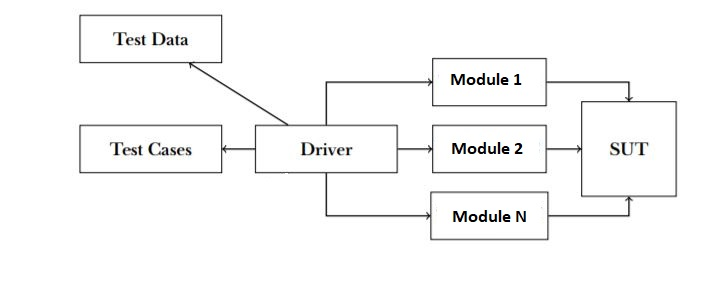
\includegraphics[width=1\textwidth]{Module.JPG}
    \caption{"Modularity Driven" testavimo vykdymo schema.}
    \label{fig:data}
\end{figure}

\newpage
\subsection{„Data Driven“ testavimas}
„Data Driven“ testavimas yra metodika, kai testavimo duomenys yra saugomi lenteliniu formatu (ODBC, CSV, Excel, SQL) - kiekvienos eilutės duomenys yra atskiras testavimo scenarijus. Šios metodikos esmė tokia, kad testavimo skriptas ima testavimo duomenis iš vieno iš paminėtų šaltinių ir įvykdo skriptą su kiekvienu duomenų rinkiniu. Paprastai testavimo skriptai naudoja duomenis, kurie yra tiesiogiai įkoduoti į skriptą, todėl norint pakartoti testą su kitais duomenimis, reikia pakeisti ir patį skriptą, todėl metodika palengvina darbą tada, kai testavimo duomenis reikia nuolat keisti  ~\cite{ORACLEHelpCenter}.

Tinkamas atvėjis, kai gali būti taikomas "Data Driven" testavimas, yra kai dviems ar daugiau testavimo scenarijų galioja tos pačios instrukcijos, bet reikalingi skirtingi įvesties parametrai ir skirtingi tikėtini rezultatai  ~\cite{ORACLEHelpCenter}.

\subsubsection{Parametrizavimas}
Parametrizavimas yra šios testavimo technikos dalis, skirta gauti duomenis iš išorinio šaltinio ir naudoti juos kaip įvesties parametrus testo programiniame kode  ~\cite{ORACLEHelpCenter}.

\subsubsection{Testavimo duomenys}
Reikia pratestuoti tinklalapio registracijos ir prisijungimo funkcionalumą, pakartoti testą naudojant skirtingus testavimo duomenis, kurie pavaizduoti žemiau.
\newline

\begin{table}[!ht]
\centering
\begin{tabular}{ |c|c|c|c|c|c|c| }
\hline
 \textbf{Vardas} & \textbf{Pavardė} & \textbf{Diena} & \textbf{Mėnesis} & \textbf{Gimimo metai} & \textbf{El. paštas} & \textbf{Slaptažodis} \\
 \hline
 Jonas & Jonaitis & 1 & 8  & 1990 & jonas@gmail.com & password \\ 
 \hline
 Lukas  & Lukaitis   & 2 & 9  & 1991 & lukas@gmail.com & password  \\ 
 \hline
 Adomas & Adomaitis  & 3 & 10 & 1992 & adomas@gmail.com & password  \\ 
 \hline
\end{tabular}
\caption{Testavimo duomenų formato pavyzdys.}
\label{table:comparison-between-approaches}
\end{table}

Žemiau pavaizduotoje schemoje egzistuoja du elementai (Žiūrėti\ \ref{fig:data}~Fig.), kurie yra būtini "Data Driven" testavimui:
\begin{itemize}
    \item \textbf{"Data Parser"}. Jis yra atsakingas už duomenų nuskaitymą iš CSV failo, duomenų bazės lentelės ar kitų šaltinių. Jo pagrindinė užduotis yra nuskaityti testams skirtus duomenis ir perduoti juos testavimo skriptui, suteikiant prieigą prie visų šaltinio duomenų.
    
    \item \textbf{"Driver Script"}. Ji yra atsakinga už bandymų vykdymo proceso naudojimą, naudojant bandymų bibliotekų teikiamas testavimo funkcijas, kurios sąveikauja su bandoma sistema ir bandymų duomenimis, kuriuos skaito duomenų analizatorius.
\end{itemize}

\begin{figure}[h]
    \centering
    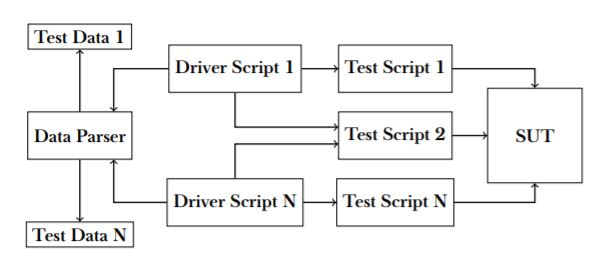
\includegraphics[width=1\textwidth]{DataDriven.JPG}
    \caption{"Data Driven" testavimo vykdymo schema.}
    \label{fig:data}
\end{figure}

\newpage
\subsubsection{Duomenų nuskaitymas iš failo}
Tam, kad atlikti „Data Driven“ testus, reikia nuskaityti duomenis iš duomenų šaltinio, tai mūsų atvėju yra Excel failas.
\begin{lstlisting}[caption={Duomenų nuskaitymas iš Excel failo.}]
    public Object[][] fetchExcelData() throws IOException {
        inputStream = getFileInputStram();
        XSSFWorkbook excelFile = new XSSFWorkbook(inputStream);
        XSSFSheet sheet = excelFile.getSheetAt(0);
        int totalNumberOfRows = sheet.getLastRowNum() + 1;
        int totalNumberOfColumns = 7;
        String[][] arrayOfExcelData = new String[totalNumberOfRows][totalNumberOfColumns];
        for (int i = 0; i < totalNumberOfRows; i++) {
            for (int j = 0; j < totalNumberOfColumns; j++) {
                XSSFRow row = sheet.getRow(i);
                arrayOfExcelData[i][j] = row.getCell(j).toString();
            }
        }
        excelFile.close();
        return arrayOfExcelData;
    }
\end{lstlisting}

% Žemiau pavaizduotoje schemoje egzistuoja du elementai (Žiūrėti\ \ref{fig:data}~Fig.), kurie yra būtini "Data Driven" testavimui:
% \begin{itemize}
%     \item \textbf{"Data Parser"}. Jis yra atsakingas už duomenų nuskaitymą iš CSV failo, duomenų bazės lentelės ar kitų šaltinių. Jo pagrindinė užduotis yra nuskaityti testams skirtus duomenis ir perduoti juos testavimo skriptui, suteikiant prieigą prie visų šaltinio duomenų.
    
%     \item \textbf{"Driver Script"}. Ji yra atsakinga už bandymų vykdymo proceso naudojimą, naudojant bandymų bibliotekų teikiamas testavimo funkcijas, kurios sąveikauja su bandoma sistema ir bandymų duomenimis, kuriuos skaito duomenų analizatorius.
% \end{itemize}

% \begin{figure}[h]
%     \centering
%     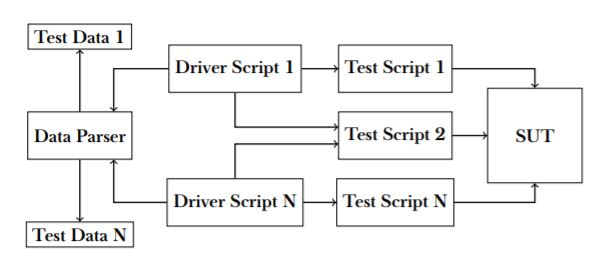
\includegraphics[width=1\textwidth]{DataDriven.JPG}
%     \caption{"Data Driven" testavimo vykdymo schema.}
%     \label{fig:data}
% \end{figure}

\newpage
\subsubsection{Testavimo scenarijaus įgyveninimas}
Vėliau iš šaltinio paimti duomenys yra naudojami atliekant testą.
\begin{lstlisting}[caption={Testo vykdymas ir parametrizacijos procesas naudojant duomenis iš Excel failo.}]
    @Test(dataProvider = "ExcelData")
    public void registrationAndLogin(String fName, String lName, String day, String month, String year, 
    String email, String password) throws InterruptedException {
        homePage = new HomePage(driver);
        userRegister = new RegistrationPage(driver);
        homePage.openRegisterationPage();
        userRegister.userRegisteration(fName, lName, day, month, year, email, password);
        Assert.assertTrue(userRegister.succesfulNotification
        .getText().contains("Your registration completed"));
        userRegister.userLogOut();
        userLogInObject = new LoginPage(driver);
        homePage.openLogInPage();
        userLogInObject.userLogIn(email, password);
        Assert.assertTrue(userRegister.logoutLink.getText()
        .contains("Log out"));
        userRegister.userLogOut();
    }
\end{lstlisting}
Ši testavimo metodika yra geriausias ir patikimiausias būdas patikrinti, kaip aplikacija elgiasi su skirtingais duomenimis, tai tikrinti kiekviename, net ir ne WEB projekte, yra būtina. Todėl testavimo procesas niekaip negali egzistuoti be šios metodikos.

\subsection{„Keyword Driven“ testavimas}
Ši automatinio testavimo atšaka yra loginis praplėtimas "Data driven" testavimo metodiką. Neskaitant testavimo duomenų, ji naudoja raktažodžius, susijusius su testuojama aplikacija. Šie raktažodžiai apibūdina veiksmų rinkinį, reikalingų atlikti tam tikrą žingsnį testavimo scenarijuje - skripte. Pirmiausia yra sukuriamas raktinių žodžių rinkinys, siejamas su tam tikru veiksmu teste. Kiekvienas bandomasis veiksmas kaip pvz. naršyklės atidarymas, naršyklės uždarymas, pelės paspaudimas yra aprašytas pasirinktu raktiniu žodžiu ~\cite{KeywordDrivenTesting}.

\subsubsection{"Keyword driven" testo duomenys}

\begin{figure}[h]
    \centering
    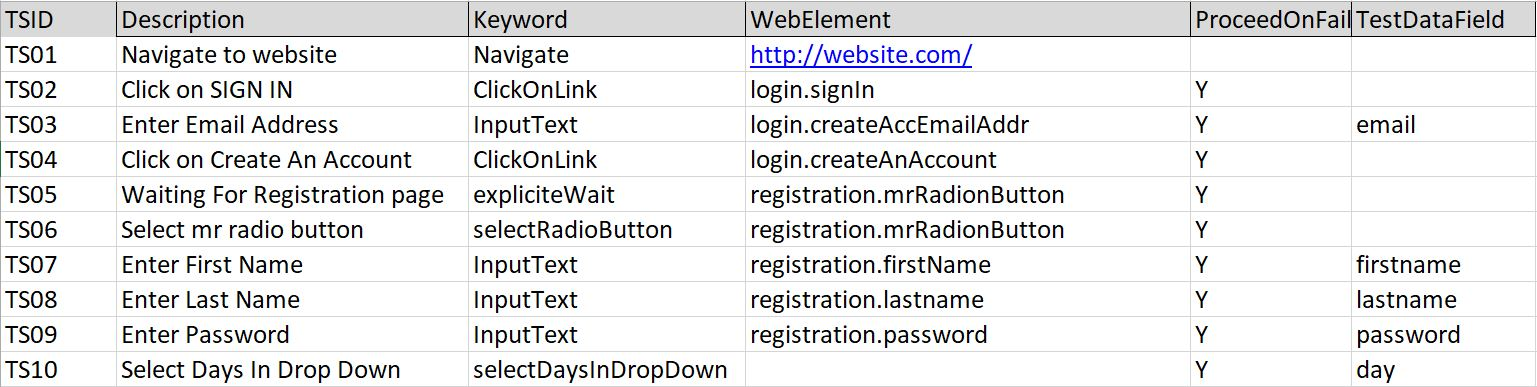
\includegraphics[width=1\textwidth]{KeywordDrivenData.JPG}
    \caption{Ištrauka iš "Keyword Driven" testavimo scenarijaus.}
    \label{fig:data}
\end{figure}

"Keyword driven" testavime yra keli elementai (Žiūrėti\ \ref{fig:keyword}~Fig.), kurie privalo būti įtraukti:
\begin{enumerate}
    \item \textbf{"Data Parser"}. Duomenų nuskaitymas iš šaltinių.
    \item \textbf{"Driver Script"}. Apdoroja raktažodžius ir duomenis, kurie reikalingi testo vykdymui.
    \item \textbf{"Handlers"}. Kiekvienas raktažodis atitinka vieną atskirą test. skripto fragmentą, jų seka (raktažodžių ir reikšmių) paverčia juos į vykdomus testus.
\end{enumerate}

\begin{figure}[h]
    \centering
    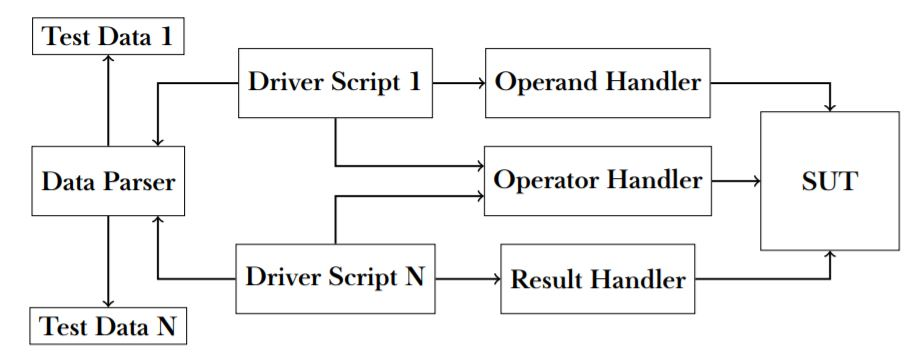
\includegraphics[width=1\textwidth]{Keyword.JPG}
    \caption{"Keyword Driven" testavimo vykdymo schema.}
    \label{fig:keyword}
\end{figure}

\subsection{„Behavior Driven“ testavimas}
Tai yra programinės įrangos plėtojimo procesas, kurio metu yra sudaromi scenarijai, kaip aplikacija turi elgtis žiūrint iš galutinio vartotojo perspektyvos. Šio testavimo tikslas - pagerinti suinteresuotųjų šalių, tokių kaip kūrėjai, testuotojai, produktų vadovai ir verslo analitikai, bendradarbiavimą, rašant testavimo scenarijus lengvai suprantama Gherkin kalba. Naudojant šią metodiką yra parašomas testavimo skriptas, fiksuojant kiekvieną testavimo žingsnį ir jį išvedant į ekraną. Šią testavimo metodiką galima įgyvendinti naudojant Cucumber, SpecFlow karkasus arba jų alternatyvas ~\cite{smart2014bdd}.

\subsubsection{Testavimo scenarijus parašytas su Gherkin}
\begin{lstlisting}[caption={Gherkin kalba parašytas testas.}]
  Scenario: Checkout a tea type
    Given I open the tea Categories Page
    When I click on the Red Tea checkout link
    And I enter name "Adomas" in the Name field
    And I enter address "Kovo g." in the Address field
    And I enter the email "adomas@gmail.com" in the email field.
    And I click submit Button
    Then I should successfully navigate to Menu page
\end{lstlisting}

Žemiau yra aprašomas testavimo scenarijus Gherkin kalba, kuri yra lengvai suprantama visiems, net ir tiem kurie neturi programavimo žinių, tačiau kiekvienas šis scenarijaus žingnis yra suprogramuotas, naudojant Selenium karkasą, taip, kaip nurodyta žemiau.

\begin{lstlisting}[caption={Gherkin testas įgyvendintas naudojant Selenium karkasą ir Java kalbą.}]
public class TeaOrder {
    ...
    @Given("^I open the tea Categories Page$")
    public void i_open_the_tea_Categories_Page(){
        hp = CheckoutUtil.openHomePage();
        tcp = hp.clickLink_Menu();
    }
    @When("^I click on the Red Tea checkout link$")
    public void i_click_on_the_Red_Tea_checkout_link(){
        cop = tcp.clickBtn_RedTea();
    }
    @When("^I enter name \"([^\"]*)\" in the Name field$")
    public void i_enter_name_in_the_Name_field(String name){
        cop.type_Txt_name(name);
    }
    @When("^I enter address \"([^\"]*)\" in the Address field$")
    public void i_enter_address_in_the_Address_field(String address){
        cop.type_Txt_address(address);
    }
    @When("^I enter the email \"([^\"]*)\" in the email field\\.$")
    public void i_enter_the_email_in_the_email_field(String email){
        cop.type_Txt_email(email);
    }
    @When("^I click submit Button$")
    public void i_click_submit_Button(){
        tcp = cop.click_Btn_Submit();
    }
    @Then("^I should successfully navigate to Menu page$")
    public void i_should_successfully_navigate_to_Menu_page(){
        Assert.assertEquals("Menu", tcp.getDriver().getTitle());
    }
    ...
    }
\end{lstlisting}

Kaip jau minėta, ši metodika palengvina komunikaciją tarp specialistų, dirbančių prie projektą, kitaip tariant - padeda "susikalbėti". "Susikalbėjimas" ir vienas kito supratimas WEB projektuose yra labai svarbus, kitaip gali būti patiriami nuostoliai, kurių 

\newpage
\subsection{„Hybrid Driven“ testavimas}
Ši testavimo metodika yra praktiškiausia ir dažniausiai sutinkama praktikoje. Ji naudoja kelias skirtingas automatinio testavimo savybes ir todėl yra vadinama "Hybrid Driven" metodika. Plačiausiai naudojama kombinacija yra testavimo projekte panaudojant "Data Driven" ir "Keyword Driven" testavimo metodikų savybes, taip kaip nurodyta schemoje apačioje (Žiūrėti\ \ref{fig:hybrid}~Fig.). Naudojant šią testavimo metodiką, kūrėjai ir testuotojai gali kompensuoti vieno automatinio testavimo tipo naudojimo trūkumus. Šis metodas yra labai tinkamas plačios apimties sistemų testavimui, kuriose yra daug duomenų rinkinių ir duomenų perkėlimo atvejų ~\cite{inproceedings}.

"Hybrid driven" testavimas naudojamas tam, kad išpildyti tokias charakteristikas kaip:
\begin{enumerate}
    \item Priežiūros paprastumas (\textbf{angl.} Maintainability)
    \item Pakartotinio panaudojamumas (\textbf{angl.} Reusability)
    \item Patikimumas
\end{enumerate}
\newline
\begin{figure}[h]
    \centering
    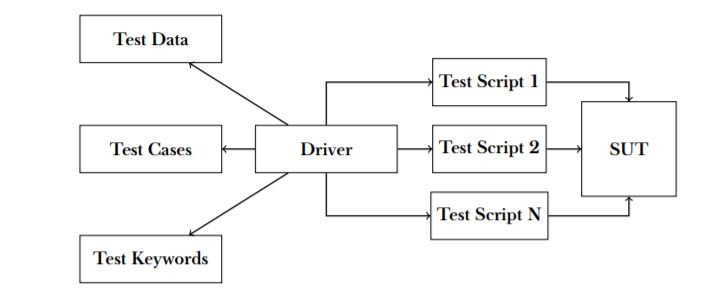
\includegraphics[width=0.8\textwidth]{Hybrid.JPG}
    \caption{"Hybrid Driven" testavimo vykdymo schema.}
    \label{fig:hybrid}
\end{figure}

Ši testavimo metodika yra pranaši tuo, kad naudojant ją testuose yra panaudojami kitų testavimo metodikų, kaip data-driven, keyword-driven ir t.t, pranašumai. Šios metodikos naudojimas žymiai sumažina riziką palikti defektų WEB ar kitokio tipo projekte,

\newpage
\section{Testavimo metodikų palyginimas}

\begin{table}[!ht]
\centering
\begin{tabular}{l|p{55mm}|p{55mm}}
\textbf{Metodika} & \textbf{Privalumai} & \textbf{Trūkumai} \\
\hline
Data driven
  & Lengva palaikyti, vykdyti testus naudojant skirtingus duomenis.
  & Norint įgyvendinti šią metodiką, reikia kvalifikuotų išteklių. \\
\hline
Keyword driven
  & Testavimo scenarijai yra suprantami ir lengvai modifikuojami, aukštas pakartotinio panaudojamumo lygis, apibrėžus raktažodžius, sudarinėti test. scenarijus gali beveik bet kas.
  & Raktinių žodžių ir susijusių funkcijų kūrimas yra daug laiko reikalaujantis procesas. \\
\hline
Hybrid driven
  & Apjungia visus automatinio \newline testavimo metodų privalumus į vieną metodą.
  & Sunkiai įgyvendinamas testavimo metodas, nes reikia išmanyti visas aut. testavimo metodikas. \\
\hline
Modularity driven
  & Sumažina kodo duplikaciją, palaiko švarų kodą, testai yra lengvai plečiami.
  & Yra mažiau veiksmingas nei kitos metodikos kaip "Keyword driven" ir "Data driven". \\
\hline
Behaviour driven
  & Palengvina bendradarbiavimą tarp visų prie produkto dirbančių specialistų, padeda susikoncentruoti ties reikalavimais.
  & \\    
\hline
Linear scripting
  & Greitas testų generavimas, \newline visiškai nereikalinga testų automatiacijos patirtis.
  & Testavimo duomenys įkoduoti į skriptą, žemas pakartotinio panaudojamumo lygis. \\
\end{tabular}
\caption{Testavimo metodikų palyginimas.}
\label{table:comparison-between-approaches}
\end{table}

 %Conclusions section
\sectionWithoutNumber{\keyWordConclusions}{conclu}
Tinkamo testavimo karkaso pasirinkimas priklauso nuo projektų, komandos patirties ir turimų išteklių ir turi didelę įtaką internetinių aplikacijų kūrimo ciklo sklandumui bei galutinio produkto kokybei, todėl ši internetinių puslapių kūrimo ciklo dalis yra gyvybiškai svarbi ir negali būti praleista. Pradedant projektą svarbu nusistatyti, į ką WEB aplikacija bus orientuota - ar tai bus aplikacija, kuri valdys didelius įvairių duomenų kiekius, ar aplikacija, kuri turės daug smulkių funkcijų, kurios yra priklausomos vienos nuo kitos ir pagal tai pasirinkti data-driven, behavior-driven ar kitokią automatinio testavimo metodiką, tačiau visgi rekomenduotina automatiniam testavimui naudoti hybrid-driven automatinio testavimo metodologiją, jungiančią daugelio metodikų privalumus į atskirą metodiką, padėsiančią užtikrinti aplikacijos kokybę vertinant ją skirtingais aspektais, kuriuos atstovauja kiekviena iš metodikų.

Tam, kad automatizacijos procesą palaikyti veiksmingą, tiek testuotojai, tiek produkto šeimininkai, vadybininkai, klientai turi norėti ir turėti galimybę atlikti pakeitimus produkte, jei to reikalauja susiklosčiusi situacija.


 %file literatureSources.bib
\referenceSources{literatureSources}

\end{document}
